\chapter{Mesh Analysis and Topology}
\label{ch:mesh_analysis}

\section{Mesh Connected Components}
\label{sec:mesh_connected_components}

\subsection{1. Overview}

Finding the \index{connected component} connected components of a mesh is the process of partitioning the mesh into sets of faces or vertices that are reachable from each other through edge connectivity. A single 3D file often often contains multiple disjoint geometric objects (e.g., a table and four separate chairs). Identifying these components is a standard preprocessing step for mesh analysis\cite{botsch2010}, repair, and selective editing.

\subsection{2. Definitions}

\begin{definition}[Connected Component]\label{def:connected_component}
A maximal subgraph of a mesh where any two nodes (vertices or faces) are connected by a path of adjacency relations.
\end{definition}

\begin{definition}[Adjacency]\label{def:mesh_adjacency}
In a mesh, two faces are \emph{edge-adjacent} if they share an edge. Two vertices are adjacent if they share an edge.
\end{definition}

\begin{definition}[Graph Traversal]\label{def:graph_traversal}
The process of visiting all reachable elements in a graph starting from a seed point, following a systematic exploration strategy such as breadth-first or depth-first search.
\end{definition}

\subsection{3. Theory}

The problem of finding connected components in a mesh is equivalent to finding the connected components of its \index{dual graph}dual graph (where nodes are faces) or its \index{primal graph}primal graph (where nodes are vertices).

\begin{theorem}[Component Count]\label{thm:component_count}
Let $M$ be a mesh with $n$ vertices and $m$ edges. The connected components of $M$ can be computed in $O(n + m)$ time using either breadth-first search or depth-first search.
\end{theorem}

\begin{proof}
Each vertex and edge is visited at most once by BFS or DFS. The algorithm maintains a set of unvisited vertices, and each vertex is removed from this set exactly once. For each vertex, all its incident edges are examined, contributing $O(\deg(v))$ work. Summing over all vertices gives $\sum_{v} O(\deg(v)) = O(m)$ by the Handshaking Lemma\cite{diestel2017}. Combined with the $O(n)$ initialization, the total is $O(n + m)$.
\end{proof}

Standard \index{breadth-first search}Breadth-First Search (BFS) or \index{depth-first search}Depth-First Search (DFS) algorithms are used:
\begin{enumerate}
    \item Initialize a set of unvisited faces.
    \item While there are unvisited faces:
    \begin{itemize}
        \item Pick an unvisited face as a ``seed.''
        \item Start a new component.
        \item Perform a BFS/DFS to find all faces reachable from the seed via shared edges.
        \item Mark all reached faces as visited and add them to the current component.
    \end{itemize}
\end{enumerate}

For manifold meshes, face-connectivity is usually sufficient. For non-manifold or point cloud data, vertex-connectivity might be required.

\begin{example}[Connected Components]\label{ex:connected_components}
Consider a mesh consisting of a tetrahedron (4 vertices, 4 faces) and a disconnected triangle (3 vertices, 1 face). The algorithm starts at an arbitrary face of the tetrahedron and discovers all 4 faces via adjacency. It then picks the lone triangle as a new seed, finding 1 face. The result is two components: one with 4 faces and one with 1 face. The Euler characteristic of the first component is $\chi_1 = 4 - 6 + 4 = 2$ (sphere-like), and the second is $\chi_2 = 3 - 3 + 1 = 1$ (disk).
\end{example}

\begin{figure}[htbp]
\centering
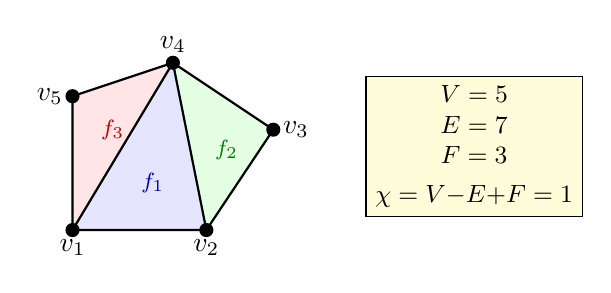
\begin{tikzpicture}[scale=0.85]
  \coordinate (v1) at (0,0);
  \coordinate (v2) at (2,0);
  \coordinate (v3) at (3,1.5);
  \coordinate (v4) at (1.5,2.5);
  \coordinate (v5) at (0,2);
  \fill[blue!10] (v1)--(v2)--(v4)--cycle;
  \fill[green!10] (v2)--(v3)--(v4)--cycle;
  \fill[red!10] (v1)--(v4)--(v5)--cycle;
  \draw[thick] (v1)--(v2) (v2)--(v3) (v3)--(v4) (v4)--(v5) (v5)--(v1);
  \draw[thick] (v1)--(v4) (v2)--(v4);
  \foreach \v/\name/\pos in {v1/$v_1$/below,v2/$v_2$/below,v3/$v_3$/right,v4/$v_4$/above,v5/$v_5$/left} {
    \fill (\v) circle (3pt) node[\pos] {\name};
  }
  \node[blue!70!black,font=\footnotesize] at (1.2,0.7) {$f_1$};
  \node[green!50!black,font=\footnotesize] at (2.3,1.2) {$f_2$};
  \node[red!70!black,font=\footnotesize] at (0.6,1.5) {$f_3$};
  \node[draw,rectangle,fill=yellow!15,font=\small,align=center] at (6,1.25) {$V=5$\\$E=7$\\$F=3$\\[3pt]$\chi = V{-}E{+}F = 1$};
\end{tikzpicture}
\caption{A triangle mesh with vertices $v_i$, edges, and faces $f_j$. The Euler characteristic $\chi = V - E + F$ is a topological invariant.}
\label{fig:mesh_connectivity}
\end{figure}


\subsection{4. Pseudocode}

\begin{algorithm}
\caption{Find Mesh Components}
\label{alg:find_mesh_components}
\begin{algorithmic}[1]
\Function{FindMeshComponents}{$mesh$}
    \State $\mathit{unvisited} \gets \text{set}(\text{range}(\mathit{num\_faces}))$
    \State $\mathit{components} \gets []$
    \While{$\mathit{unvisited}$}
        \State $\mathit{seed} \gets \mathit{unvisited}.\text{pop}()$
        \State $\mathit{current\_component} \gets [\mathit{seed}]$
        \State $\mathit{queue} \gets [\mathit{seed}]$
        \While{$\mathit{queue}$}
            \State $f \gets \mathit{queue}.\text{pop}(0)$
            \For{$\mathit{neighbor} \in \text{GetAdjacentFaces}(f, mesh)$}
                \If{$\mathit{neighbor} \in \mathit{unvisited}$}
                    \State $\mathit{unvisited}.\text{remove}(\mathit{neighbor})$
                    \State $\mathit{current\_component}.\text{append}(\mathit{neighbor})$
                    \State $\mathit{queue}.\text{append}(\mathit{neighbor})$
                \EndIf
            \EndFor
        \EndWhile
        \State $\mathit{components}.\text{append}(\mathit{current\_component})$
    \EndWhile
    \State \Return $\mathit{components}$
\EndFunction
\end{algorithmic}
\end{algorithm}

\subsection{5. Parameter Selection}

\begin{itemize}
    \item \textbf{Connectivity Type}: \textbf{Edge-connectivity} (faces sharing an edge) is standard. \textbf{Vertex-connectivity} (faces sharing only a vertex) is ``weaker'' and will result in fewer, larger components.
    \item \textbf{Data Structure}: Using a \index{half-edge}Half-Edge\cite{guibas1985} structure or an \index{adjacency list}Adjacency List makes finding neighbors $O(1)$, leading to optimal performance.
\end{itemize}

\subsection{6. Complexity}

\begin{itemize}
    \item \textbf{Time Complexity}: $O(F)$ where $F$ is the number of faces, as each face and each adjacency relationship is visited a constant number of times.
    \item \textbf{Space Complexity}: $O(F)$ to store the visited status and the resulting component lists.
\end{itemize}

\subsection{7. Usages}

\begin{itemize}
    \item \textbf{Mesh Repair}: Identifying and removing small ``floating'' noise components (e.g., isolated triangles) from a scan.
    \item \textbf{Selective Editing}: Selecting an entire object by clicking on a single triangle (e.g., ``Select Linked'' in Blender).
    \item \textbf{3D Printing}: Ensuring that a model consists of a single connected ``shell'' or identifying internal voids.
    \item \textbf{Rigging and Animation}: Automatically grouping parts of a character (e.g., separating the body from the clothing or eyes).
    \item \textbf{Physics Simulation}: Treating each connected component as a separate rigid body for collision and dynamics.
\end{itemize}

\subsection{8. Testing Methods and Edge Cases}

\begin{itemize}
    \item \textbf{Single Watertight Object}: Should return exactly one component containing all faces.
    \item \textbf{Disconnected Objects}: Verify that multiple separate objects are correctly identified as distinct components.
    \item \textbf{Points/Lines}: Ensure the algorithm handles ``degenerate'' components like isolated vertices or edges.
    \item \textbf{Non-Manifold Edges}: Verify that connectivity is correctly traced even if three or more faces share an edge.
    \item \textbf{Large Meshes}: Test performance on meshes with millions of triangles to ensure linear scaling.
\end{itemize}

\subsection{9. References}

\begin{itemize}
    \item Hopcroft, J., \& Tarjan, R. (1973). ``Efficient algorithms for graph manipulation.'' Communications of the ACM.
    \item Botsch, M., Kobbelt, L., Pauly, M., Alliez, P., \& L\'evy, B. \cite{botsch2010} ``Polygon Mesh Processing.'' CRC Press.
    \item Wikipedia: Connected component (graph theory).
\end{itemize}

\section{Mesh Boundary Detection}
\label{sec:mesh_boundary_detection}

\subsection{1. Overview}

Mesh \index{boundary detection}boundary detection is the process of identifying vertices and edges that form the boundary\index{boundary edge} of a surface mesh\cite{botsch2010}. In a manifold mesh, every edge is shared by exactly two faces. Boundary edges are those that are part of only one face. Identifying these boundaries is essential for surface parameterization, texture mapping, and mesh editing.

\subsection{2. Definitions}

\begin{definition}[Surface Mesh]\label{def:surface_mesh}
A collection of vertices, edges, and faces that represent a 2-dimensional surface embedded in 3-dimensional space.
\end{definition}

\begin{definition}[Boundary Edge]\label{def:boundary_edge}
An edge that is incident to exactly one face. In a half-edge data structure\cite{guibas1985}, this corresponds to a half-edge whose \texttt{twin} is null.
\end{definition}

\begin{definition}[Boundary Vertex]\label{def:boundary_vertex}
A vertex that is incident to at least one boundary edge.
\end{definition}

\begin{definition}[Boundary Loop]\label{def:boundary_loop}
A connected cycle of boundary edges and vertices that define a hole or the perimeter of the mesh.
\end{definition}

\subsection{3. Theory}

The fundamental principle of mesh boundary detection is counting the \index{face-edge incidence}face-edge incidence. For a given mesh $M$ with $F$ faces:
\begin{enumerate}
    \item Iterate through all faces.
    \item For each face, extract its oriented edges (e.g., $(v_1, v_2), (v_2, v_3), (v_3, v_1)$).
    \item Store the occurrence of each edge in a hash map, ignoring the orientation (i.e., $(v_i, v_j)$ is the same as $(v_j, v_i)$).
    \item Edges that appear only \textbf{once} in the total count are boundary edges.
\end{enumerate}

\begin{theorem}[Boundary Edge Characterization]\label{thm:boundary_edge_char}
In a closed 2-manifold mesh, every edge is shared by exactly two faces. An edge $e$ is a boundary edge if and only if it is incident to exactly one face.
\end{theorem}

\begin{proof}
By definition of a 2-manifold with boundary, each edge is incident to either one face (boundary edge) or two faces (interior edge). The edge count algorithm enumerates all face-edge incidences. An interior edge appears twice (once per adjacent face), while a boundary edge appears exactly once. Hence, edges with count equal to 1 are precisely the boundary edges.
\end{proof}

Once the boundary edges are identified, they can be chained together by matching endpoints to form one or more \index{boundary loop}boundary loops.

\begin{example}[Boundary Detection]\label{ex:boundary_detection}
Consider a single triangle with vertices $(v_0, v_1, v_2)$ and edges $\{(v_0,v_1), (v_1,v_2), (v_2,v_0)\}$. The edge count map stores each edge with count 1. All three edges are boundary edges, and chaining them produces a single boundary loop $(v_0, v_1, v_2)$. For a tetrahedron (4 triangles), every edge is shared by exactly 2 faces, so the count is always 2 and no boundary edges are found.
\end{example}

\subsection{4. Pseudocode}

\begin{algorithm}
\caption{Detect Mesh Boundaries}
\label{alg:detect_mesh_boundaries}
\begin{algorithmic}[1]
\Function{DetectMeshBoundaries}{$mesh$}
    \State $\mathit{edge\_counts} \gets \{\}$
    \For{$\mathit{face} \in mesh.\mathit{faces}$}
        \For{$i = 0 \to \text{len}(\mathit{face}) - 1$}
            \State $v_1, v_2 \gets \text{SortedPair}(\mathit{face}[i], \mathit{face}[(i+1) \bmod \text{len}(\mathit{face})])$
            \State $\mathit{edge\_counts}[(v_1, v_2)] \gets \mathit{edge\_counts}.get((v_1, v_2), 0) + 1$
        \EndFor
    \EndFor
    \State $\mathit{boundary\_edges} \gets [e \mid e, c \in \mathit{edge\_counts}.items() \text{ if } c = 1]$
    \State $\mathit{loops} \gets []$
    \State $\mathit{visited\_edges} \gets \{\}$
    \For{$\mathit{start\_edge} \in \mathit{boundary\_edges}$}
        \If{$\mathit{start\_edge} \in \mathit{visited\_edges}$}
            \State \textbf{continue}
        \EndIf
        \State $\mathit{current\_loop} \gets [\mathit{start\_edge}[0], \mathit{start\_edge}[1]]$
        \State $\mathit{visited\_edges}.\text{add}(\mathit{start\_edge})$
        \While{True}
            \State $\mathit{next\_edge} \gets \text{FindNextBoundaryEdge}(\mathit{current\_loop}[-1], \mathit{boundary\_edges}, \mathit{visited\_edges})$
            \If{$\mathit{next\_edge} = \textbf{None}$ or $\mathit{next\_edge} = \mathit{start\_edge}$}
                \State \textbf{break}
            \EndIf
            \State $\mathit{next\_v} \gets \mathit{next\_edge}[1]$ if $\mathit{next\_edge}[0] = \mathit{current\_loop}[-1]$ \textbf{else} $\mathit{next\_edge}[0]$
            \State $\mathit{current\_loop}.\text{append}(\mathit{next\_v})$
            \State $\mathit{visited\_edges}.\text{add}(\mathit{next\_edge})$
        \EndWhile
        \State $\mathit{loops}.\text{append}(\mathit{current\_loop})$
    \EndFor
    \State \Return $\mathit{loops}$
\EndFunction
\end{algorithmic}
\end{algorithm}

\subsection{5. Parameter Selection}

\begin{itemize}
    \item \textbf{Mesh Representation}: Using a \index{half-edge}Half-Edge\cite{guibas1985} data structure makes boundary detection trivial, as boundary edges are typically stored as ``null'' half-edges or explicit boundary objects.
    \item \textbf{Sorting}: When using an indexed face set, sorting the vertex IDs for each edge (e.g., $(\min(u,v), \max(u,v))$) ensures that the count correctly accounts for both orientations of the same geometric edge.
\end{itemize}

\subsection{6. Complexity}

\begin{itemize}
    \item \textbf{Time Complexity}: $O(F)$, where $F$ is the number of faces in the mesh. Chaining the loops takes $O(E_{\text{boundary}})$.
    \item \textbf{Space Complexity}: $O(E)$ to store the edge counts.
\end{itemize}

\subsection{7. Usages}

\begin{itemize}
    \item \textbf{Surface Parameterization (UV Mapping)}: BFF and Harmonic Mapping require the mesh boundary to be identified and mapped to a 2D shape.
    \item \textbf{Mesh Repair}: Identifying and filling holes in scanned 3D models.
    \item \textbf{Texture Blending}: Applying effects specifically at the boundaries of different surface materials.
    \item \textbf{Physical Simulation}: Applying boundary conditions (like fixing a boundary in place) for Finite Element analysis.
\end{itemize}

\subsection{8. Testing Methods and Edge Cases}

\begin{itemize}
    \item \textbf{Watertight Mesh}: A perfectly closed mesh (like a sphere) should return zero boundary edges.
    \item \textbf{Open Sheet}: A mesh like a flat square should return a single boundary loop containing all perimeter edges.
    \item \textbf{Non-Manifold Edges}: Edges shared by more than two faces (count $> 2$) should be flagged as errors or handled separately.
    \item \textbf{Duplicate Faces}: Two faces covering the same three vertices will result in edge counts of 2, making them appear ``watertight'' even if they are isolated.
    \item \textbf{Multiple Holes}: Verify that each hole is correctly identified as a separate loop.
\end{itemize}

\subsection{9. References}

\begin{itemize}
    \item Botsch, M., Kobbelt, L., Pauly, M., Alliez, P., \& L\'evy, B. \cite{botsch2010} ``Polygon Mesh Processing.'' CRC Press.
    \item Guibas, L. J., \& Stolfi, J. \cite{guibas1985} ``Primitives for the manipulation of general subdivisions.'' ACM Transactions on Graphics.
    \item Wikipedia: Boundary (topology).
\end{itemize}

\section{Mesh Orientability}
\label{sec:mesh_orientability}

\subsection{1. Overview}

Mesh \index{orientability}orientability is a property of a surface mesh that determines whether a consistent ``outside'' and ``inside'' (or a consistent normal direction) can be defined for the entire surface. An orientable surface allows every face to be oriented so that any two adjacent faces share an edge with opposite orientations. Non-orientable surfaces, such as the M\"obius strip or the Klein bottle, cannot be assigned a consistent orientation\cite{botsch2010}.

\subsection{2. Definitions}

\begin{definition}[Face Orientation]\label{def:face_orientation}
The order in which the vertices of a face are listed (e.g., $(v_1, v_2, v_3)$), which determines the face normal using the right-hand rule.
\end{definition}

\begin{definition}[Orientable Surface]\label{def:orientable_surface}
A surface where face orientations can be made consistent: for every edge shared by faces $F_1$ and $F_2$, the orientations of $F_1$ and $F_2$ must traverse the edge in opposite directions.
\end{definition}

\begin{definition}[Inconsistent Edge]\label{def:inconsistent_edge}
An edge where both incident faces traverse the edge in the same direction (e.g., both use $(u, v)$).
\end{definition}

\begin{definition}[Two-Sided Surface]\label{def:two_sided}
An orientable manifold mesh effectively has two sides (e.g., the inside and outside of a sphere).
\end{definition}

\subsection{3. Theory}

The process of orienting a mesh is a \index{graph search}graph-search problem.
\begin{enumerate}
    \item Represent the mesh as a \index{dual graph}dual graph where each node is a face and edges connect adjacent faces (those sharing an edge).
    \item Select an initial face and assign it an arbitrary orientation (e.g., CCW).
    \item Propagate this orientation to its neighbors: if face $F_1$ uses edge $(u, v)$, then its neighbor $F_2$ \textbf{must} use edge $(v, u)$.
    \item If at any point we encounter a neighbor that has already been oriented in a way that conflicts with its current neighbor, the mesh is \textbf{non-orientable}.
\end{enumerate}

\begin{theorem}[Orientability Characterization]\label{thm:orientability}
A connected 2-manifold surface $S$ is orientable if and only if it does not contain a M\"obius strip as a sub-surface. Equivalently, $S$ is orientable if and only if every edge is traversed by its two incident faces in opposite directions.
\end{theorem}

\begin{proof}
If $S$ is orientable, we can assign consistent face orientations, so every edge is traversed in opposite directions by its two incident faces. Conversely, if every edge is traversed in opposite directions, the BFS propagation never encounters a conflict, and we obtain a consistent global orientation. The non-orientable case requires the existence of an orientation-reversing cycle, which is topologically equivalent to a M\"obius strip.
\end{proof}

Mathematically, a manifold surface is orientable if and only if it does not contain a M\"obius strip as a sub-surface.

\begin{example}[Orienting a Triangle Mesh]\label{ex:orient_mesh}
Consider a tetrahedron with faces $F_1 = (v_0,v_1,v_2)$, $F_2 = (v_0,v_2,v_3)$, $F_3 = (v_0,v_3,v_1)$, $F_4 = (v_1,v_3,v_2)$. Starting at $F_1$ with CCW orientation, edge $(v_0,v_2)$ is traversed from $v_0$ to $v_2$. Face $F_2$ must then traverse this edge as $(v_2,v_0)$, which is satisfied by $(v_0,v_2,v_3)$. Propagating to $F_3$ via edge $(v_0,v_3)$, we require $(v_3,v_0)$, satisfied by $(v_0,v_3,v_1)$. All four faces receive consistent orientations, confirming the tetrahedron is orientable.
\end{example}

\subsection{4. Pseudocode}

\begin{algorithm}
\caption{Orient Mesh}
\label{alg:orient_mesh}
\begin{algorithmic}[1]
\Function{OrientMesh}{$mesh$}
    \State $\mathit{oriented\_faces} \gets \{\}$
    \State $\mathit{face\_directions} \gets \{\}$
    \For{$\mathit{start\_face} \in mesh.\mathit{faces}$}
        \If{$\mathit{start\_face} \in \mathit{oriented\_faces}$}
            \State \textbf{continue}
        \EndIf
        \State $\mathit{queue} \gets [\mathit{start\_face}]$
        \State $\mathit{oriented\_faces}.\text{add}(\mathit{start\_face})$
        \While{$\mathit{queue}$}
            \State $\mathit{current\_face} \gets \mathit{queue}.\text{pop}(0)$
            \For{$(\mathit{neighbor\_face}, \mathit{shared\_edge}) \in \text{GetNeighbors}(\mathit{current\_face}, mesh)$}
                \If{$\mathit{neighbor\_face} \notin \mathit{oriented\_faces}$}
                    \State $\mathit{new\_orientation} \gets \text{MatchOrientation}(\mathit{current\_face}, \mathit{neighbor\_face}, \mathit{shared\_edge})$
                    \State $\mathit{face\_directions}[\mathit{neighbor\_face}] \gets \mathit{new\_orientation}$
                    \State $\mathit{oriented\_faces}.\text{add}(\mathit{neighbor\_face})$
                    \State $\mathit{queue}.\text{append}(\mathit{neighbor\_face})$
                \Else
                    \If{$\neg \text{IsConsistent}(\mathit{current\_face}, \mathit{neighbor\_face}, \mathit{shared\_edge})$}
                        \State \Return \textbf{False}, ``Mesh is non-orientable (M\"obius strip topology)''
                    \EndIf
                \EndIf
            \EndFor
        \EndWhile
    \EndFor
    \State \Return \textbf{True}, $\mathit{face\_directions}$
\EndFunction

\Statex

\Function{IsConsistent}{$f_1, f_2, edge$}
    \State $u, v \gets \text{GetEdgeVertices}(f_1, edge)$
    \State $u', v' \gets \text{GetEdgeVertices}(f_2, edge)$
    \State \Return $(u = v') \wedge (v = u')$
\EndFunction
\end{algorithmic}
\end{algorithm}

\subsection{5. Parameter Selection}

\begin{itemize}
    \item \textbf{Start Face}: Any face can be used as a starting point. For non-closed meshes, starting at a boundary can be helpful.
    \item \textbf{Components}: Orientation must be checked and performed independently for each connected component of the mesh.
\end{itemize}

\subsection{6. Complexity}

\begin{itemize}
    \item \textbf{Time Complexity}: $O(F)$, where $F$ is the number of faces, as each face is visited exactly once in the BFS.
    \item \textbf{Space Complexity}: $O(F)$ to store the face orientations and the BFS queue.
\end{itemize}

\subsection{7. Usages}

\begin{itemize}
    \item \textbf{Rendering}: Backface culling and lighting calculations depend on correct, consistent normals.
    \item \textbf{Slicing for 3D Printing}: Determining what is ``solid'' vs ``void'' requires consistent orientations.
    \item \textbf{Surface Offsetting}: Offsetting a surface requires moving vertices in a consistent normal direction.
    \item \textbf{Fluid Simulation}: Pressure forces must be applied consistently along the surface normals.
\end{itemize}

\subsection{8. Testing Methods and Edge Cases}

\begin{itemize}
    \item \textbf{M\"obius Strip}: A classic non-orientable manifold; the algorithm should detect the inconsistency.
    \item \textbf{Klein Bottle}: A closed non-orientable surface (though it must self-intersect in 3D).
    \item \textbf{Watertight Sphere}: Orienting one face should correctly orient the entire sphere.
    \item \textbf{Disconnected Mesh}: Ensure the algorithm handles multiple separate objects in the same file.
    \item \textbf{Non-Manifold Mesh}: Orientability is generally defined for manifolds; non-manifold edges (shared by 3+ faces) make orientability ambiguous.
\end{itemize}

\subsection{9. References}

\begin{itemize}
    \item Botsch, M., Kobbelt, L., Pauly, M., Alliez, P., \& L\'evy, B. \cite{botsch2010} ``Polygon Mesh Processing.'' CRC Press.
    \item Guibas, L. J., \& Stolfi, J. \cite{guibas1985} ``Primitives for the manipulation of general subdivisions.'' ACM Transactions on Graphics.
    \item Wikipedia: Orientability.
\end{itemize}

\section{Manifold Verification}
\label{sec:manifold_verification}

\subsection{1. Overview}

\index{manifold verification}Manifold verification is the process of checking whether a 3D surface mesh satisfies the topological constraints of a 2nd-order manifold. A \index{manifold}manifold surface is one that ``locally looks like a flat plane'' at every point. Manifold meshes are highly desirable in geometric modeling because they have well-defined orientations, consistent normals, and are compatible with standard data structures like the half-edge mesh\cite{guibas1985}.

\subsection{2. Definitions}

\begin{definition}[Edge Manifold]\label{def:edge_manifold}
An edge is \emph{edge-manifold} if it is shared by exactly two faces (for a closed surface) or one face (for a boundary edge).
\end{definition}

\begin{definition}[Vertex Manifold]\label{def:vertex_manifold}
A vertex is \emph{vertex-manifold} if its surrounding faces form a single, connected ``fan'' or ``disk.''
\end{definition}

\begin{definition}[Watertight]\label{def:watertight}
A closed manifold mesh with no holes: every edge has exactly two incident faces. Equivalently, the mesh has no boundary edges.
\end{definition}

\begin{definition}[Euler Characteristic]\label{def:euler_char_manifold}
For a manifold mesh with $V$ vertices, $E$ edges, and $F$ faces, the \index{Euler characteristic}Euler characteristic is $\chi = V - E + F$. For a sphere-like surface, $\chi = 2$.
\end{definition}

\subsection{3. Theory}

To verify that a mesh is a manifold, we check three primary conditions\cite{botsch2010}:
\begin{enumerate}
    \item \textbf{Edge Condition}: Every edge must be incident to either one or two faces. Edges with three or more incident faces (non-manifold edges) are topologically ambiguous.
    \item \textbf{Vertex Condition}: For each vertex, the set of faces sharing that vertex must be edge-connected. If a vertex belongs to two separate ``cones'' that only touch at the vertex itself, it is non-manifold.
    \item \textbf{Face Consistency}: For each edge, the orientation of its two incident faces must be compatible (e.g., if one face uses $(u, v)$, the other must use $(v, u)$).
\end{enumerate}

\begin{theorem}[Manifold Verification Correctness]\label{thm:manifold_correctness}
A mesh $M$ is a 2-manifold if and only if it satisfies the edge condition, the vertex condition, and the face consistency condition simultaneously.
\end{theorem}

\begin{proof}
($\Rightarrow$) If $M$ is a 2-manifold, then by definition every point has a neighborhood homeomorphic to a half-plane (boundary) or full plane (interior). This implies each edge has at most two incident faces (edge condition), each vertex has a single fan of faces (vertex condition), and the orientations are globally consistent (face consistency).

($\Leftarrow$) If all three conditions hold, the BFS orientation propagation succeeds globally (face consistency). The edge condition ensures no edge has more than two faces. The vertex condition ensures each vertex has a single connected neighborhood. Together, these guarantee that every point has the required local topological structure.
\end{proof}

\begin{figure}[htbp]
\centering
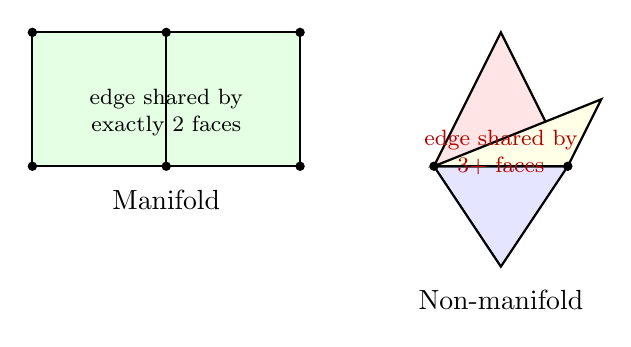
\begin{tikzpicture}[scale=0.85]
  \begin{scope}[xshift=-3cm]
    \draw[thick,fill=green!10] (0,0)--(2,0)--(2,2)--(0,2)--cycle;
    \draw[thick,fill=green!10] (2,0)--(4,0)--(4,2)--(2,2)--cycle;
    \fill (0,0) circle (2pt); \fill (2,0) circle (2pt); \fill (4,0) circle (2pt);
    \fill (0,2) circle (2pt); \fill (2,2) circle (2pt); \fill (4,2) circle (2pt);
    \node at (2,-0.5) {Manifold};
    \node[font=\footnotesize] at (2,1) {edge shared by};
    \node[font=\footnotesize] at (2,0.6) {exactly 2 faces};
  \end{scope}
  \begin{scope}[xshift=3cm]
    \draw[thick,fill=red!10] (0,0)--(2,0)--(1,2)--cycle;
    \draw[thick,fill=blue!10] (0,0)--(2,0)--(1,-1.5)--cycle;
    \draw[thick,fill=yellow!10] (0,0)--(2,0)--(2.5,1)--cycle;
    \fill (0,0) circle (2pt); \fill (2,0) circle (2pt);
    \node at (1,-2) {Non-manifold};
    \node[font=\footnotesize,red!70!black] at (1,0.4) {edge shared by};
    \node[font=\footnotesize,red!70!black] at (1,0) {3+ faces};
  \end{scope}
\end{tikzpicture}
\caption{(Left)~Manifold mesh: every edge is shared by exactly two faces. (Right)~Non-manifold: an edge shared by three faces violates the manifold property.}
\label{fig:manifold}
\end{figure}


\subsection{4. Pseudocode}

\begin{algorithm}
\caption{Is Manifold}
\label{alg:is_manifold}
\begin{algorithmic}[1]
\Function{IsManifold}{$mesh$}
    \State $\mathit{edge\_faces} \gets \text{GetEdgeFaceMap}(mesh)$
    \For{$(\mathit{edge}, \mathit{faces}) \in \mathit{edge\_faces}.\text{items}()$}
        \If{$\text{len}(\mathit{faces}) > 2$}
            \State \Return \textbf{False}, ``Non-manifold edge detected''
        \EndIf
    \EndFor
    \For{$\mathit{vertex} \in mesh.\mathit{vertices}$}
        \State $\mathit{neighbor\_faces} \gets \text{GetFacesSharingVertex}(\mathit{vertex}, mesh)$
        \If{$\neg \text{IsConnected}(\mathit{neighbor\_faces}, \mathit{vertex})$}
            \State \Return \textbf{False}, ``Non-manifold vertex detected''
        \EndIf
    \EndFor
    \If{$\neg \text{HasConsistentOrientation}(mesh)$}
        \State \Return \textbf{False}, ``Inconsistent face orientations''
    \EndIf
    \State \Return \textbf{True}, ``Mesh is manifold''
\EndFunction

\Statex

\Function{IsConnected}{$faces, vertex$}
    \State $\mathit{components} \gets \text{FindFaceComponents}(faces, vertex)$
    \State \Return $\text{len}(\mathit{components}) = 1$
\EndFunction
\end{algorithmic}
\end{algorithm}

\subsection{5. Parameter Selection}

\begin{itemize}
    \item \textbf{Tolerance}: Floating-point precision should be considered when identifying ``duplicate'' vertices that should have been merged.
    \item \textbf{Boundary Handling}: A manifold with a boundary is still a manifold; the condition for boundary edges (1 face) and boundary vertices (faces form a single half-disk) must be handled.
\end{itemize}

\subsection{6. Complexity}

\begin{itemize}
    \item \textbf{Time Complexity}: $O(F)$, where $F$ is the number of faces, to build the edge-face map and check vertex connectivity.
    \item \textbf{Space Complexity}: $O(E + F)$ to store the connectivity information.
\end{itemize}

\subsection{7. Usages}

\begin{itemize}
    \item \textbf{3D Printing}: Slicing software requires watertight, manifold meshes to correctly identify ``inside'' vs.\ ``outside'' volumes.
    \item \textbf{Physical Simulation}: Finite Element Method (FEM) and Fluid Dynamics simulations often fail on non-manifold geometry.
    \item \textbf{Mesh Boolean Operations}: Algorithms like Union/Intersection are much more robust on manifold meshes.
    \item \textbf{Surface Parameterization}: Algorithms like BFF or LSCM rely on a consistent half-edge structure, which requires a manifold mesh.
\end{itemize}

\subsection{8. Testing Methods and Edge Cases}

\begin{itemize}
    \item \textbf{T-Junctions}: A vertex lying on an edge of another face (without sharing it) is geometrically non-manifold.
    \item \textbf{Pinch Points}: Two separate mesh components touching at a single vertex.
    \item \textbf{Self-Intersections}: A mesh can be topologically manifold while still being geometrically self-intersecting (this is usually checked separately).
    \item \textbf{Isolated Vertices}: Vertices with zero incident faces.
    \item \textbf{Inconsistent Normals}: A ``M\"obius strip'' style mesh where orientations cannot be made consistent.
\end{itemize}

\subsection{9. References}

\begin{itemize}
    \item Guibas, L. J., \& Stolfi, J. \cite{guibas1985} ``Primitives for the manipulation of general subdivisions.'' ACM Transactions on Graphics.
    \item Botsch, M., Kobbelt, L., Pauly, M., Alliez, P., \& L\'evy, B. \cite{botsch2010} ``Polygon Mesh Processing.'' CRC Press.
    \item Wikipedia: Manifold.
\end{itemize}

\section{Euler Characteristic}
\label{sec:euler_characteristic}

\subsection{1. Overview}

The \index{Euler characteristic}Euler characteristic ($\chi$) is a topological invariant, a number that describes a topological space's shape or structure regardless of the way it is bent or twisted. For a 3D surface mesh (a polyhedral surface), it relates the number of vertices ($V$), edges ($E$), and faces ($F$). It is a fundamental tool for classifying surfaces and verifying the topological integrity of meshes\cite{euler1758,poincare1895}.

\subsection{2. Definitions}

\begin{definition}[Euler Formula]\label{def:euler_formula}
For a convex polyhedron (topologically equivalent to a sphere), the \index{Euler formula}Euler formula states that $\chi = V - E + F = 2$.
\end{definition}

\begin{definition}[Genus]\label{def:genus}
The \index{genus}genus $g$ of a surface is the number of ``handles'' or ``holes'' through a surface (e.g., a torus has $g=1$, a sphere has $g=0$).
\end{definition}

\begin{definition}[Boundary Components]\label{def:boundary_components}
The number $b$ of connected boundary loops in a mesh.
\end{definition}

\begin{definition}[Topological Invariant]\label{def:topological_invariant}
A property that remains unchanged under continuous deformation (homeomorphism).
\end{definition}

\subsection{3. Theory}

For a general connected orientable surface, the Euler characteristic is related to its genus and boundary count by the formula:
$$\chi = V - E + F = 2 - 2g - b$$

\begin{theorem}[Euler--Poincar\'e Formula]\label{thm:euler_poincare}
For a connected orientable 2-manifold with genus $g$ and $b$ boundary components, the Euler characteristic satisfies $\chi = V - E + F = 2 - 2g - b$. In particular, for a closed surface ($b = 0$), $\chi = 2 - 2g$.
\end{theorem}

\begin{proof}
We prove this by induction on the genus $g$. For $g = 0$ (a sphere), the classical Euler formula gives $\chi = 2$. We establish the formula for $g = 0, b > 0$ by noting that each boundary component is obtained by removing a disk, which reduces $\chi$ by 1. Hence $\chi = 2 - b$.

For the inductive step, suppose the formula holds for genus $g$. To obtain a surface of genus $g+1$, we remove two disks from the surface and attach a cylinder (tube) between the resulting boundary circles. Removing two disks decreases $\chi$ by 2, and attaching the cylinder (which has $\chi = 0$) does not change $\chi$. The genus increases by 1. Thus $\chi_{g+1} = \chi_g - 2 = (2 - 2g) - 2 = 2 - 2(g+1)$, completing the induction.
\end{proof}

This allows us to determine the global topology of a mesh simply by counting its elements:
\begin{itemize}
    \item \textbf{Sphere}: $V - E + F = 2$ ($g=0, b=0$).
    \item \textbf{Disk}: $V - E + F = 1$ ($g=0, b=1$).
    \item \textbf{Torus}: $V - E + F = 0$ ($g=1, b=0$).
    \item \textbf{Cylinder}: $V - E + F = 0$ ($g=0, b=2$).
\end{itemize}

The \index{Gauss--Bonnet theorem}Gauss--Bonnet theorem further relates the Euler characteristic to the total curvature of the surface: $\int_M K \, dA = 2\pi \chi$. In the discrete case, this means the sum of angle defects at all vertices is exactly $2\pi \chi$, where the angle defect at vertex $v$ is defined as $\delta(v) = 2\pi - \sum_{i} \theta_i$, with $\theta_i$ being the angles of the faces incident to $v$.

\begin{example}[Euler Characteristic Computations]\label{ex:euler_characteristic}
\begin{enumerate}
    \item \textbf{Tetrahedron}: $V = 4$, $E = 6$, $F = 4$. Thus $\chi = 4 - 6 + 4 = 2$, confirming it is homeomorphic to a sphere ($g = 0$).
    \item \textbf{Cube}: $V = 8$, $E = 12$, $F = 6$. Thus $\chi = 8 - 12 + 6 = 2$.
    \item \textbf{Torus (mesh approximation)}: A torus mesh with $V$ vertices satisfies $V - E + F = 0$, regardless of resolution. For instance, a coarse torus with $V = 16$, $E = 32$, $F = 16$ gives $\chi = 0$.
    \item \textbf{Two disjoint spheres}: $V = 8$, $E = 12$, $F = 8$ (two tetrahedra). $\chi = 8 - 12 + 8 = 4 = 2 \times 2$, consistent with the formula for $C = 2$ components.
\end{enumerate}
\end{example}

\subsection{4. Pseudocode}

\begin{algorithm}
\caption{Calculate Euler Characteristic}
\label{alg:calculate_euler_characteristic}
\begin{algorithmic}[1]
\Function{CalculateEulerCharacteristic}{$mesh$}
    \State $V \gets \text{len}(mesh.\mathit{vertices})$
    \State $F \gets \text{len}(mesh.\mathit{faces})$
    \State $\mathit{edges} \gets \{\}$
    \For{$\mathit{face} \in mesh.\mathit{faces}$}
        \For{$i = 0 \to \text{len}(\mathit{face}) - 1$}
            \State $v_1 \gets \mathit{face}[i]$
            \State $v_2 \gets \mathit{face}[(i+1) \bmod \text{len}(\mathit{face})]$
            \State $\mathit{edges}.\text{add}(\text{tuple}(\text{sorted}((v_1, v_2))))$
        \EndFor
    \EndFor
    \State $E \gets \text{len}(\mathit{edges})$
    \State $\chi \gets V - E + F$
    \State \Return $\chi$
\EndFunction
\end{algorithmic}
\end{algorithm}

\subsection{5. Parameter Selection}

\begin{itemize}
    \item \textbf{Element Counting}: Ensure that duplicate vertices or edges are correctly merged before counting, as they will artificially deflate/inflate $\chi$.
    \item \textbf{Component Handling}: If the mesh has $C$ disconnected components, the formula becomes $\chi = V - E + F = 2C - 2g - b$.
\end{itemize}

\subsection{6. Complexity}

\begin{itemize}
    \item \textbf{Time Complexity}: $O(F)$, where $F$ is the number of faces, to iterate through the mesh and identify unique edges.
    \item \textbf{Space Complexity}: $O(E)$ to store the set of unique edges.
\end{itemize}

\subsection{7. Usages}

\begin{itemize}
    \item \textbf{Mesh Verification}: Detecting if a mesh has unexpected holes or disconnected parts.
    \item \textbf{Surface Classification}: Automatically determining if a scanned object is a ``donut'' (torus) or a ``ball'' (sphere).
    \item \textbf{Topology-Preserving Operations}: Ensuring that operations like mesh simplification or remeshing do not change the number of holes in the model.
    \item \textbf{Shape Matching}: Using $\chi$ as a fast, first-pass filter to distinguish between objects with different topologies.
    \item \textbf{Theoretical Physics}: Used in string theory and condensed matter physics to classify manifold structures.
\end{itemize}

\subsection{8. Testing Methods and Edge Cases}

\begin{itemize}
    \item \textbf{Platonic Solids}: Verify that the Tetrahedron, Cube, Octahedron, Dodecahedron, and Icosahedron all yield $\chi = 2$.
    \item \textbf{Open Meshes}: A single triangle has $V=3, E=3, F=1 \Rightarrow \chi=1$ (a disk).
    \item \textbf{Disconnected Parts}: A mesh consisting of two separate spheres should have $\chi = 4$.
    \item \textbf{Non-Orientable Surfaces}: For a M\"obius strip, $\chi = 0$ ($V-E+F = 0$, $g_{\text{non-orient}}=1, b=1$).
    \item \textbf{Non-Manifold Edges}: Ensure the edge counting logic correctly handles edges shared by 3+ faces (though the standard formula is defined for 2-manifolds).
\end{itemize}

\subsection{9. References}

\begin{itemize}
    \item Euler, L. \cite{euler1758} ``Elementa doctrinae solidorum.'' Novi Commentarii Academiae Scientiarum Petropolitanae.
    \item Poincar\'e, H. \cite{poincare1895} ``Analysis situs.'' Journal de l'\'Ecole Polytechnique.
    \item Botsch, M., Kobbelt, L., Pauly, M., Alliez, P., \& L\'evy, B. \cite{botsch2010} ``Polygon Mesh Processing.'' CRC Press.
    \item Wikipedia: Euler characteristic.
\end{itemize}

\section{Node Degree and Valence}
\label{sec:node_degree}

\subsection{1. Overview}

Node degree calculation is the process of counting the number of edges incident to each vertex (node) in a graph or mesh. In the context of 3D meshes, vertex degree (often called \index{valence}\textbf{valence}) is a key indicator of mesh quality and topological regularity. Vertices with unusual degrees (extraordinary vertices\index{extraordinary vertex}) can cause artifacts in subdivision and smoothing algorithms\cite{botsch2010}.

\subsection{2. Definitions}

\begin{definition}[Valence (Degree)]\label{def:valence}
The number of edges connected to a vertex $v$, denoted $\deg(v)$.
\end{definition}

\begin{definition}[Regular Vertex]\label{def:regular_vertex}
A vertex with the ``ideal'' degree for its mesh type: degree 6 for triangle meshes, degree 4 for quad meshes.
\end{definition}

\begin{definition}[Extraordinary Vertex]\label{def:extraordinary_vertex}
A vertex with a degree other than the regular degree. Also called a \index{singularity}singularity.
\end{definition}

\begin{definition}[Average Degree]\label{def:average_degree}
The sum of all degrees divided by the number of vertices. For a closed triangle mesh, the average degree approaches 6 as $V \to \infty$.
\end{definition}

\subsection{3. Theory}

\begin{theorem}[Handshaking Lemma]\label{thm:handshaking}
The sum of all vertex degrees in a mesh is equal to twice the number of edges: $\sum_{i=1}^{V} \deg(v_i) = 2E$.
\end{theorem}

\begin{proof}
Each edge $(u, v)$ contributes exactly 1 to $\deg(u)$ and 1 to $\deg(v)$. Summing over all edges, the total contribution to the degree sum is $2E$.
\end{proof}

For a closed 2-manifold triangle mesh, the average degree is related to the \index{Euler characteristic}Euler characteristic $\chi$:
$$\bar{d} = 6 - \frac{6\chi}{V}$$

\begin{theorem}[Average Degree of Triangle Mesh]\label{thm:avg_degree}
For a closed 2-manifold triangle mesh with $V$ vertices, $E$ edges, and Euler characteristic $\chi$, the average vertex degree is $\bar{d} = 6 - 6\chi / V$.
\end{theorem}

\begin{proof}
By the Handshaking Lemma\cite{diestel2017}, $\bar{d} = 2E / V$. For a triangle mesh, each face has 3 edges and each edge is shared by 2 faces, so $3F = 2E$, giving $F = 2E/3$. Substituting into Euler's formula $\chi = V - E + F$:
$$\chi = V - E + \frac{2E}{3} = V - \frac{E}{3}$$
Hence $E = 3(V - \chi)$, and $\bar{d} = 2E/V = 6(V - \chi)/V = 6 - 6\chi/V$.
\end{proof}

As the number of vertices $V \to \infty$, the average degree approaches 6.

In a \index{half-edge}Half-Edge\cite{guibas1985} data structure, calculating the degree involves ``circulating'' around the vertex using the \texttt{next} and \texttt{twin} pointers until the starting half-edge is reached again.

\begin{example}[Valence Distribution]\label{ex:valence_distribution}
Consider an icosahedron: $V = 12$, $E = 30$, $F = 20$. Every vertex has degree 5 (all vertices are regular for this polyhedron). The average degree is $\bar{d} = 2 \times 30 / 12 = 5$, which matches the formula $\bar{d} = 6 - 6(2)/12 = 5$. In a refined triangle mesh with genus 0 and many vertices, the average degree approaches 6, but the 12 original icosahedral vertices remain extraordinary with degree 5.
\end{example}

\subsection{4. Pseudocode}

\textbf{Using an Adjacency List:}

\begin{algorithm}
\caption{Calculate Vertex Degrees}
\label{alg:calculate_degrees}
\begin{algorithmic}[1]
\Function{CalculateDegrees}{$mesh$}
    \State $\mathit{degrees} \gets [0] \times \mathit{num\_vertices}$
    \For{$(v_1, v_2) \in mesh.\mathit{edges}$}
        \State $\mathit{degrees}[v_1] \gets \mathit{degrees}[v_1] + 1$
        \State $\mathit{degrees}[v_2] \gets \mathit{degrees}[v_2] + 1$
    \EndFor
    \State \Return $\mathit{degrees}$
\EndFunction
\end{algorithmic}
\end{algorithm}

\textbf{Using a Half-Edge Structure:}

\begin{algorithm}
\caption{Get Vertex Degree}
\label{alg:get_vertex_degree}
\begin{algorithmic}[1]
\Function{GetVertexDegree}{$mesh, v$}
    \State $\mathit{count} \gets 0$
    \State $\mathit{start\_he} \gets v.\mathit{halfedge}$
    \State $\mathit{curr\_he} \gets \mathit{start\_he}$
    \Loop
        \State $\mathit{count} \gets \mathit{count} + 1$
        \State $\mathit{curr\_he} \gets \mathit{curr\_he}.\mathit{twin}.\mathit{next}$
        \If{$\mathit{curr\_he} = \mathit{start\_he}$}
            \State \textbf{break}
        \EndIf
    \EndLoop
    \State \Return $\mathit{count}$
\EndFunction
\end{algorithmic}
\end{algorithm}

\subsection{5. Parameter Selection}

\begin{itemize}
    \item \textbf{Boundary Handling}: Vertices on the boundary of an open mesh naturally have lower degrees (typically 2 or 3). They should be flagged or handled separately in quality metrics.
    \item \textbf{Directed vs.\ Undirected}: For general graphs, degrees are split into \textbf{In-Degree} and \textbf{Out-Degree}. For standard surface meshes, edges are considered undirected.
\end{itemize}

\subsection{6. Complexity}

\begin{itemize}
    \item \textbf{Time Complexity}: $O(E)$ to iterate through all edges, or $O(V \cdot \bar{d})$ to circulate around each vertex. Both are linear in the size of the mesh.
    \item \textbf{Space Complexity}: $O(V)$ to store the degree values.
\end{itemize}

\subsection{7. Usages}

\begin{itemize}
    \item \textbf{Mesh Quality Analysis}: Identifying regions with poor connectivity that might cause simulation errors.
    \item \textbf{Subdivision Surfaces}: Stencils for \index{Loop subdivision}Loop\cite{loop1987} or \index{Catmull-Clark subdivision}Catmull-Clark\cite{catmull1978} subdivision change based on the vertex degree to maintain smoothness.
    \item \textbf{Mesh Simplification}: Algorithms like Quadratic Error Metrics (QEM) often prioritize removing vertices based on their degree and geometric impact.
    \item \textbf{Network Science}: Identifying ``hubs'' (nodes with very high degrees) in social or infrastructure graphs.
    \item \textbf{Topology Verification}: Checking if a mesh is ``regular'' (e.g., all vertices have degree 6).
\end{itemize}

\subsection{8. Testing Methods and Edge Cases}

\begin{itemize}
    \item \textbf{Simple Polyhedra}: Verify that all vertices of a cube have degree 3, and all vertices of an icosahedron have degree 5.
    \item \textbf{Regular Grid}: A flat triangle grid should have interior vertices of degree 6.
    \item \textbf{Boundary Vertices}: Test on an open square; corner vertices should have degree 2 and edge vertices degree 3.
    \item \textbf{Non-Manifold Vertices}: Verify the count when multiple ``fans'' of triangles meet at a single vertex.
    \item \textbf{Isolated Vertices}: Ensure vertices with zero edges are handled (degree 0).
\end{itemize}

\subsection{9. References}

\begin{itemize}
    \item Diestel, R. \cite{diestel2017} ``Graph Theory.'' Springer.
    \item Botsch, M., Kobbelt, L., Pauly, M., Alliez, P., \& L\'evy, B. \cite{botsch2010} ``Polygon Mesh Processing.'' CRC Press.
    \item Wikipedia: Degree (graph theory).
\end{itemize}

\section{Mesh Coloring}
\label{sec:mesh_coloring}

\subsection{1. Overview}

Mesh \index{graph coloring}coloring is the process of assigning labels (colors) to the elements of a mesh (typically vertices or faces) such that no two adjacent elements share the same label. This is a direct application of graph coloring to the connectivity of a mesh. While it is often used for visual aesthetics, its primary technical purpose is to identify independent sets of elements that can be processed in parallel without race conditions.

\subsection{2. Definitions}

\begin{definition}[$k$-Coloring]\label{def:k_coloring}
An assignment of $k$ colors to vertices such that adjacent vertices have different colors.
\end{definition}

\begin{definition}[Vertex Graph]\label{def:vertex_graph}
A graph where vertices of the mesh are nodes and edges of the mesh are graph edges.
\end{definition}

\begin{definition}[Dual Graph (Face Graph)]\label{def:dual_graph_coloring}
A graph where each face of the mesh is a node and edges connect faces that share an edge.
\end{definition}

\begin{definition}[Chromatic Number]\label{def:chromatic_number}
The \index{chromatic number}chromatic number $\chi(G)$ is the minimum number of colors needed to color a graph $G$.
\end{definition}

\subsection{3. Theory}

For a 2D surface mesh (which is essentially a planar or surface-embedded graph), several key theorems apply:

\begin{theorem}[Four-Color Theorem]\label{thm:four_color}
Any planar graph can be colored with at most 4 colors\cite{welsh1967}. Since most surface meshes are locally planar, 4 to 6 colors are typically sufficient.
\end{theorem}

\begin{proof}
The Four-Color Theorem was originally proved by Appel and Haken (1976) using computer-assisted case analysis, and later given a simpler (though still computer-assisted) proof by Robertson, Sanders, Seymour, and Thomas (1997). The key idea is that every planar graph has a vertex of degree at most 5, which allows an inductive argument: remove such a vertex, color the smaller graph by induction, then restore the vertex using one of the 4 colors not used by its at-most-5 neighbors (by the pigeonhole principle, at least one color is available among 4). The hard part is handling the finite set of unavoidable configurations.
\end{proof}

\begin{theorem}[Brooks' Theorem]\label{thm:brooks}
The chromatic number is at most the maximum vertex degree $\Delta$, unless the graph is a complete graph or an odd cycle.
\end{theorem}

The most common algorithm is the \index{greedy coloring}\textbf{Greedy Coloring} approach:
\begin{enumerate}
    \item Iterate through vertices in a specific order.
    \item For the current vertex, check the colors of its already-colored neighbors.
    \item Assign the smallest available color that is not used by any neighbor.
\end{enumerate}

\begin{example}[Greedy Coloring Trace]\label{ex:greedy_coloring}
Consider a triangle mesh with vertices $v_0, v_1, v_2, v_3$ forming two triangles $(v_0,v_1,v_2)$ and $(v_1,v_2,v_3)$. Ordering by descending degree: $v_1$ (deg 4), $v_2$ (deg 4), $v_0$ (deg 2), $v_3$ (deg 2). Color $v_1$ with 0 (no colored neighbors). Color $v_2$ with 1 (neighbor $v_1$ uses 0). Color $v_0$ with 1 (neighbors $v_1$ uses 0, $v_2$ uses 1; but $v_0$ is only adjacent to $v_1$ and $v_2$). Wait, $v_0$ is adjacent to both $v_1$ and $v_2$ in triangle $(v_0,v_1,v_2)$, so its neighbors use colors $\{0,1\}$; assign color 2. Color $v_3$ similarly with color 2 (neighbors $v_1$ and $v_2$ use $\{0,1\}$). Total: 3 colors, matching the fact that the chromatic number of a triangle mesh is at most 4 by \cref{thm:four_color}.
\end{example}

\subsection{4. Pseudocode}

\begin{algorithm}
\caption{Color Mesh}
\label{alg:color_mesh}
\begin{algorithmic}[1]
\Function{ColorMesh}{$mesh$, \textit{strategy} = ``GREEDY''}
    \State $\mathit{colors} \gets \{v : -1 \mid v \in mesh.\mathit{vertices}\}$
    \State $\mathit{ordered\_vertices} \gets \text{SortByDegree}(mesh.\mathit{vertices}, \textit{descending} = \textbf{True})$
    \For{$v \in \mathit{ordered\_vertices}$}
        \State $\mathit{neighbor\_colors} \gets \{\}$
        \For{$\mathit{neighbor} \in \text{GetNeighbors}(v, mesh)$}
            \If{$\mathit{colors}[\mathit{neighbor}] \neq -1$}
                \State $\mathit{neighbor\_colors}.\text{add}(\mathit{colors}[\mathit{neighbor}])$
            \EndIf
        \EndFor
        \State $\mathit{color} \gets 0$
        \While{$\mathit{color} \in \mathit{neighbor\_colors}$}
            \State $\mathit{color} \gets \mathit{color} + 1$
        \EndWhile
        \State $\mathit{colors}[v] \gets \mathit{color}$
    \EndFor
    \State \Return $\mathit{colors}$
\EndFunction
\end{algorithmic}
\end{algorithm}

\subsection{5. Parameter Selection}

\begin{itemize}
    \item \textbf{Ordering Strategy}: Sorting vertices by degree (Largest First) often results in fewer total colors than a random ordering.
    \item \textbf{Saturation Degree (DSATUR)}: A more advanced strategy that colors vertices with the most uniquely colored neighbors first.
\end{itemize}

\subsection{6. Complexity}

\begin{itemize}
    \item \textbf{Time Complexity}: $O(V \cdot \Delta)$, where $V$ is the number of vertices and $\Delta$ is the average vertex degree (typically $\Delta \approx 6$ for triangular meshes).
    \item \textbf{Space Complexity}: $O(V)$ to store the assigned color for each vertex.
\end{itemize}

\subsection{7. Usages}

\begin{itemize}
    \item \textbf{Parallel Computing (GPGPU)}: When performing operations like mesh smoothing (Mean Curvature Flow\cite{gage1986,grayson1987}) on a GPU, vertices of the same color can be updated simultaneously because they don't share data with each other.
    \item \textbf{Implicit Solvers}: Partitioning the Laplacian matrix into independent blocks for faster parallel solves.
    \item \textbf{Visualizing Mesh Structure}: Highlighting different regions or patches for debugging.
    \item \textbf{Texture Mapping}: Assigning different texture atlases to different parts of a mesh to avoid overlaps.
\end{itemize}

\subsection{8. Testing Methods and Edge Cases}

\begin{itemize}
    \item \textbf{Adjacency Check}: After coloring, iterate through every edge $(u, v)$ and verify that $\text{color}[u] \neq \text{color}[v]$.
    \item \textbf{Color Count}: Verify that the total number of colors used is reasonably small (e.g., $< 10$ for typical meshes).
    \item \textbf{Disconnected Components}: Ensure the algorithm handles multiple separate mesh objects correctly.
    \item \textbf{High-Valence Vertices}: Check performance and color count on meshes with ``star'' patterns (vertices with many neighbors).
    \item \textbf{Face Coloring}: Test by applying the same logic to the dual graph (coloring faces instead of vertices).
\end{itemize}

\subsection{9. References}

\begin{itemize}
    \item Welsh, D. J. A., \& Powell, M. B. \cite{welsh1967} ``An upper bound for the chromatic number of a graph and its application to timetabling problems.'' The Computer Journal.
    \item Br\'elaz, D. (1979). ``New methods to color the vertices of a graph.'' Communications of the ACM.
    \item Wikipedia: Graph coloring.
\end{itemize}

\section{Mesh Reordering}
\label{sec:mesh_reordering}

\subsection{1. Overview}

Mesh reordering is the process of permuting the indices of the vertices (and faces) of a mesh to improve the performance of numerical solvers and data access patterns. The most common objective is to minimize the \index{bandwidth}\textbf{bandwidth} of the sparse matrices derived from the mesh (like the Laplacian). Reducing the bandwidth ensures that non-zero entries are clustered close to the main diagonal, leading to faster computations and more efficient CPU cache usage\cite{cuthill1969}.

\subsection{2. Definitions}

\begin{definition}[Bandwidth]\label{def:bandwidth}
For a matrix $A$, the bandwidth is the maximum value of $|i - j|$ such that $A_{ij} \ne 0$.
\end{definition}

\begin{definition}[Permutation]\label{def:permutation}
A mapping $P$ that reassigns each vertex index $i$ to a new index $j = P(i)$.
\end{definition}

\begin{definition}[Profile]\label{def:matrix_profile}
The total number of zeros within the band of the matrix; smaller profiles are generally better.
\end{definition}

\begin{definition}[Adjacency Graph]\label{def:adjacency_graph}
The graph where vertices of the mesh are nodes and edges represent connections between them.
\end{definition}

\subsection{3. Theory}

The most widely used reordering technique is the \index{Reverse Cuthill--McKee}Reverse Cuthill--McKee (RCM) algorithm\cite{cuthill1969}. It is a refinement of a breadth-first search (BFS) that carefully chooses the starting node and the order of neighbors.

\begin{enumerate}
    \item Find a ``pseudo-peripheral'' vertex (one that is far from other vertices, often by using a heuristic).
    \item Perform a BFS starting from this vertex.
    \item In each step of the BFS, sort the neighbors by their degree (number of connections) in ascending order.
    \item Once all vertices are visited, reverse the resulting permutation. Reversing is key because it significantly reduces the matrix profile compared to the standard CM order.
\end{enumerate}

\begin{example}[RCM Reordering]\label{ex:rcm_reordering}
Consider a path graph $v_0 - v_1 - v_2 - v_3 - v_4$. Starting BFS from the peripheral vertex $v_0$: the permutation is $[v_0, v_1, v_2, v_3, v_4]$. Reversing gives $[v_4, v_3, v_2, v_1, v_0]$. The bandwidth of the adjacency matrix is 1 in both cases (since it is already optimal for a path). However, for a more complex mesh like a 2D grid, RCM produces a bandwidth of $O(\sqrt{N})$ rather than $O(N)$.
\end{example}

\subsection{4. Pseudocode}

\begin{algorithm}
\caption{RCM Reorder}
\label{alg:rcm_reorder}
\begin{algorithmic}[1]
\Function{RCMReorder}{$mesh$}
    \State $v \gets \text{FindPseudoPeripheralVertex}(mesh)$
    \State $R \gets [v]$
    \State $\mathit{visited} \gets \{v\}$
    \For{$\mathit{current\_v} \in R$}
        \State $\mathit{neighbors} \gets \text{GetNeighbors}(\mathit{current\_v}, mesh)$
        \State $\mathit{sorted\_neighbors} \gets \text{sorted}([n \mid n \in \mathit{neighbors} \text{ if } n \notin \mathit{visited}], \textit{key} = \lambda \, n : \text{len}(\text{GetNeighbors}(n, mesh)))$
        \For{$n \in \mathit{sorted\_neighbors}$}
            \State $R.\text{append}(n)$
            \State $\mathit{visited}.\text{add}(n)$
        \EndFor
    \EndFor
    \State \Return $\text{list}(\text{reversed}(R))$
\EndFunction
\end{algorithmic}
\end{algorithm}

\subsection{5. Parameter Selection}

\begin{itemize}
    \item \textbf{Starting Vertex}: The choice of the first vertex is critical. A bad starting point leads to high bandwidth. Heuristics like the Gibbs--Poole--Stockmeyer (GPS) algorithm are often used to find a good starting point.
    \item \textbf{Metric}: While bandwidth reduction is the most common goal, other orderings (like Nested Dissection) are better for parallel solvers or multifrontal methods.
\end{itemize}

\subsection{6. Complexity}

\begin{itemize}
    \item \textbf{Time Complexity}: $O(V \cdot \Delta \log \Delta)$, where $V$ is vertices and $\Delta$ is average degree. Since $\Delta \approx 6$ for meshes, this is essentially $O(V)$.
    \item \textbf{Space Complexity}: $O(V + E)$ to store the adjacency list and the visit status.
\end{itemize}

\subsection{7. Usages}

\begin{itemize}
    \item \textbf{Sparse Linear Solvers}: Essential preprocessing step for Cholesky or LU factorization of Laplacian systems.
    \item \textbf{FEM Simulations}: Reducing memory access time and improving cache hit rates in structural or fluid simulations.
    \item \textbf{Data Compression}: Reordered meshes often have more predictable connectivity, allowing for better compression (e.g., in the PLY or OBJ formats).
    \item \textbf{Rendering}: Improving the vertex cache hit rate during triangle strip or fan rendering.
\end{itemize}

\subsection{8. Testing Methods and Edge Cases}

\begin{itemize}
    \item \textbf{Bandwidth Calculation}: Compare the bandwidth of the Laplacian matrix before and after reordering. A successful RCM should show a significant reduction.
    \item \textbf{Graph with Disconnected Components}: The algorithm must be applied to each component separately and concatenated.
    \item \textbf{Highly Regular Mesh}: A perfect grid should be reordered into a diagonal-like pattern.
    \item \textbf{Very Large Mesh}: Ensure the algorithm handles millions of vertices without excessive memory overhead.
    \item \textbf{Degenerate Mesh}: Test on meshes with very high-valence vertices (where bandwidth reduction is harder).
\end{itemize}

\subsection{9. References}

\begin{itemize}
    \item Cuthill, E., \& McKee, J. \cite{cuthill1969} ``Reducing the bandwidth of sparse symmetric matrices.'' ACM National Conference.
    \item George, A. (1971). ``Computer implementation of the finite element method.'' Stanford Technical Report.
    \item Liu, W. H., \& Sherman, A. H. (1976). ``Comparative analysis of the Cuthill--McKee and the reverse Cuthill--McKee algorithms for sparse matrices.'' SIAM Journal on Numerical Analysis.
    \item Wikipedia: Cuthill--McKee algorithm.
\end{itemize}

\section{Mesh Rigidity}
\label{sec:mesh_rigidity}

\subsection{1. Overview}

Mesh rigidity is the study of whether a framework of vertices and edges (a mesh) can be continuously deformed while preserving the lengths of all its edges. A mesh is \textbf{rigid} if the only possible motions are rigid body motions (translation and rotation). If it can be deformed in other ways, it is \textbf{flexible}. Rigidity analysis is critical for structural engineering, robotics, and molecular biology.

\subsection{2. Definitions}

\begin{definition}[Bar-and-Joint Framework]\label{def:bar_joint}
A graph where edges represent rigid bars and vertices represent flexible joints.
\end{definition}

\begin{definition}[Rigidity Matrix]\label{def:rigidity_matrix}
A matrix $R$ that relates the velocities of vertices to the rates of change of edge lengths. For each edge $(i,j)$, the corresponding row contains $(P_i - P_j)$ at columns $3i$ through $3i+2$ and $(P_j - P_i)$ at columns $3j$ through $3j+2$.
\end{definition}

\begin{definition}[Infinitesimal Rigidity]\label{def:infinitesimal_rigidity}
A linear approximation where a mesh is rigid if the only vertex velocities that preserve edge lengths (to first order) are rigid body motions.
\end{definition}

\begin{definition}[Degrees of Freedom]\label{def:dof}
The dimension of the kernel of the rigidity matrix. For a rigid 3D framework, $\text{DOF} = 6$ (3 translation + 3 rotation).
\end{definition}

\subsection{3. Theory}

The rigidity of a mesh is determined by the \textbf{Rigidity Matrix} $R$. For each edge $(i, j)$, there is a row in $R$ containing the vector $(P_i - P_j)$ at columns corresponding to $P_i$ and $(P_j - P_i)$ at columns for $P_j$.

A framework is infinitesimally rigid if the rank of $R$ is $3V - 6$ (in 3D) or $2V - 3$ (in 2D).
\begin{itemize}
    \item If $\text{rank}(R) < 3V - 6$, the mesh has internal mechanisms (it is flexible).
    \item If $\text{rank}(R) = 3V - 6$, the mesh is rigid.
    \item If the number of edges $E > 3V - 6$, the mesh is \textbf{redundantly rigid} or over-constrained.
\end{itemize}

\begin{theorem}[Maxwell's Counting Rule / Laman's Theorem in 2D]\label{thm:laman}
A graph $G = (V, E)$ in 2D is generically rigid if and only if $E = 2V - 3$ and for every subgraph $H = (V', E')$ with $|V'| \geq 2$, $E' \leq 2|V'| - 3$.
\end{theorem}

\begin{proof}
The necessity direction is straightforward: if $E > 2|V'| - 3$ for some subgraph, then that subgraph has too few constraints relative to its vertices, so it must be flexible. The sufficiency direction (the harder direction) was proved by Laman\cite{laman1970} using a combinatorial characterization based on matroid theory. The key insight is that the generic rigidity matroid on a graph $G$ coincides with the sparsity matroid defined by the counting condition, which can be checked efficiently using the pebble game algorithm.
\end{proof}

\textbf{Maxwell's Counting Rule} provides a combinatorial necessary condition: a graph must have at least $3V-6$ edges to be rigid in 3D, but this is not sufficient (as the edges might be poorly distributed).

\begin{example}[Rigidity Analysis]\label{ex:rigidity}
\begin{enumerate}
    \item \textbf{Tetrahedron}: $V = 4$, $E = 6$, $3V - 6 = 6$. The rigidity matrix has rank 6, so the tetrahedron is rigid. It is the simplest rigid 3D structure.
    \item \textbf{Square with no diagonal}: $V = 4$, $E = 4$, $3V - 6 = 6$. Since $E < 3V - 6$, the square is under-constrained and flexible (it can be deformed into a rhombus). Adding one diagonal gives $E = 5 < 6$, still flexible. Adding both diagonals gives $E = 6 = 3V - 6$, and the resulting framework is rigid.
    \item \textbf{Icosahedron}: $V = 12$, $E = 30$, $3V - 6 = 30$. Exactly the right count, and the icosahedron is rigid.
\end{enumerate}
\end{example}

\subsection{4. Pseudocode}

\begin{algorithm}
\caption{Analyze Mesh Rigidity}
\label{alg:analyze_mesh_rigidity}
\begin{algorithmic}[1]
\Function{AnalyzeMeshRigidity}{$mesh$}
    \State $V \gets \text{len}(mesh.\mathit{vertices})$
    \State $E \gets \text{len}(mesh.\mathit{edges})$
    \If{$E < 3 \cdot V - 6$}
        \State \Return ``Flexible (under-constrained)''
    \EndIf
    \State $R \gets \text{SparseMatrix}(E, 3 \cdot V)$
    \For{$(\mathit{row\_idx}, \mathit{edge}) \in \text{enumerate}(mesh.\mathit{edges})$}
        \State $i, j \gets \mathit{edge}$
        \State $p_i \gets mesh.\mathit{vertices}[i]$
        \State $p_j \gets mesh.\mathit{vertices}[j]$
        \State $\mathit{diff} \gets p_i - p_j$
        \State $R[\mathit{row\_idx}, 3i : 3i+3] \gets \mathit{diff}$
        \State $R[\mathit{row\_idx}, 3j : 3j+3] \gets -\mathit{diff}$
    \EndFor
    \State $\mathit{rank} \gets \text{CalculateRank}(R)$
    \State $\mathit{dof} \gets 3 \cdot V - \mathit{rank}$
    \If{$\mathit{dof} = 6$}
        \State \Return ``Rigid''
    \Else
        \State \Return ``Flexible with $\mathit{dof} - 6$ internal mechanisms''
    \EndIf
\EndFunction
\end{algorithmic}
\end{algorithm}

\subsection{5. Parameter Selection}

\begin{itemize}
    \item \textbf{Numerical Tolerance}: Since rank calculation is sensitive to noise, a threshold based on the machine epsilon or the smallest non-zero singular value must be used.
    \item \textbf{Generic vs.\ Specific Position}: A mesh might be rigid in general but flexible in a specific degenerate configuration (e.g., all vertices on a line). Generic rigidity depends only on the graph topology.
\end{itemize}

\subsection{6. Complexity}

\begin{itemize}
    \item \textbf{Matrix Construction}: $O(E)$.
    \item \textbf{Rank Calculation}: $O(E \cdot V^2)$ using SVD. For large meshes, sparse solvers or \textbf{Pebble Game} algorithms (for combinatorial rigidity) are used.
\end{itemize}

\subsection{7. Usages}

\begin{itemize}
    \item \textbf{Structural Engineering}: Verifying that a bridge or building truss is stable and won't collapse.
    \item \textbf{Robotics}: Analyzing the workspace and mobility of parallel manipulators.
    \item \textbf{Molecular Biology}: Studying the flexibility of protein structures to understand how they bind to other molecules.
    \item \textbf{Sensor Networks}: Determining if a set of distance measurements is sufficient to uniquely locate all sensors (Localization).
    \item \textbf{Computer Graphics}: Constraining mesh deformations to be ``as-rigid-as-possible'' (ARAP) for realistic animation.
\end{itemize}

\subsection{8. Testing Methods and Edge Cases}

\begin{itemize}
    \item \textbf{Tetrahedron}: The simplest rigid 3D structure ($V=4, E=6, 3V-6=6$).
    \item \textbf{Square}: A 2D square with 4 edges is flexible ($V=4, E=4, 2V-3=5$ required); adding a diagonal makes it rigid.
    \item \textbf{Collinear Vertices}: Verify that the algorithm detects flexibility when vertices are aligned, even if the graph is combinatorially rigid.
    \item \textbf{Disconnected Mesh}: The rank check should reflect the sum of rigid body motions for each component (6 DOF per component).
    \item \textbf{Over-constrained Mesh}: Ensure the algorithm handles $E > 3V-6$ correctly.
\end{itemize}

\subsection{9. References}

\begin{itemize}
    \item Asimow, L., \& Roth, B. (1978). ``The rigidity of graphs.'' Transactions of the American Mathematical Society.
    \item Laman, G. \cite{laman1970} ``On graphs and rigidity of plane skeletal structures.'' Journal of Engineering Mathematics.
    \item Connelly, R. (1980). ``The rigidity of polyhedra.'' SIAM Journal on Mathematical Analysis.
    \item Wikipedia: Structural rigidity.
\end{itemize}

\section{Mesh Decimation via Quadric Error Metrics}
\label{sec:mesh_decimation_qem}

\subsection{1. Overview}

\index{mesh decimation}Mesh decimation is the process of reducing the number of faces (and vertices) in a triangle mesh while preserving its geometric shape as closely as possible. This is a fundamental operation in computer graphics and geometric computing. High-resolution meshes captured by 3D scanners or generated by subdivision surfaces often contain millions of triangles, far more than necessary for real-time rendering, transmission, or simulation. Mesh decimation enables \index{level of detail}Level-of-Detail (LOD) management, where coarser versions of a model are used when it occupies a small portion of the screen, and finer versions when it is viewed up close. Other critical applications include reducing the cost of \index{finite element method}Finite Element Method (FEM) simulations, accelerating ray tracing, and lowering memory and bandwidth requirements for networked 3D applications.

The \index{quadric error metric}Quadric Error Metric (QEM) method, introduced by Garland and Heckbert \cite{garland1997}, is one of the most widely used decimation algorithms. It proceeds by iteratively collapsing edges, where each collapse merges two vertices into one. The key insight is that the geometric error introduced by an edge collapse can be efficiently approximated using $4 \times 4$ symmetric matrices called \emph{quadrics}, enabling near-optimal vertex placement at each step.

\subsection{2. Definitions}

\begin{definition}[Edge Collapse]\label{def:edge_collapse}
An \index{edge collapse}edge collapse is an operation that merges two adjacent vertices $u$ and $v$ into a single vertex $\bar{v}$, removing the edge $(u, v)$ and all faces incident to it. Formally, the map $u \mapsto \bar{v}$, $v \mapsto \bar{v}$ is applied to all faces, and degenerate faces (those with fewer than three distinct vertices) are discarded.
\end{definition}

\begin{definition}[Quadric Error Metric]\label{def:quadric_error_metric}
Given a vertex $v$, its \index{quadric}quadric matrix $Q_v$ is a $4 \times 4$ symmetric matrix that summarizes the squared distances from $v$ to a set of planes. For a point $\bar{v}$ in homogeneous coordinates $\bar{v}_h = (\bar{v}_x, \bar{v}_y, \bar{v}_z, 1)^\top$, the quadric error is $\Delta(\bar{v}) = \bar{v}_h^\top \, Q_v \, \bar{v}_h$. The quadric for a single plane $\mathbf{p} = (a, b, c, d)^\top$ (where $a^2 + b^2 + c^2 = 1$) is $K_\mathbf{p} = \mathbf{p} \, \mathbf{p}^\top$.
\end{definition}

\begin{definition}[Link Condition]\label{def:link_condition}
The \index{link condition}link of a vertex $v$, denoted $\operatorname{Link}(v)$, is the set of edges connecting the neighbors of $v$ that are not incident to $v$ itself. An edge $(u, v)$ satisfies the link condition if $\operatorname{Link}(u) \cap \operatorname{Link}(v) \subseteq \operatorname{Link}(u, v)$, where $\operatorname{Link}(u, v)$ is the set of edges in the link of both $u$ and $v$ that are not the edge $(u, v)$ itself. This condition ensures that the local topology is consistent after the collapse.
\end{definition}

\begin{definition}[Manifold Preservation]\label{def:manifold_preservation}
A decimation step \emph{preserves manifoldness} if, after the edge collapse, every edge remains incident to at most two faces and every vertex retains a single connected fan of incident faces.
\end{definition}

\subsection{3. Theory}

The QEM algorithm assigns each vertex $v$ a $4 \times 4$ symmetric matrix $Q_v$ that encodes the sum of squared distances from $v$ to the planes of all faces incident to $v$.

\subsubsection{Initial Quadric Computation}

For each face with unit outward normal $\mathbf{n} = (n_x, n_y, n_z)^\top$ and offset $d = -\mathbf{n} \cdot \mathbf{v}_0$ (where $\mathbf{v}_0$ is any vertex of the face), define the plane vector $\mathbf{p} = (n_x, n_y, n_z, d)^\top$. The \index{fundamental quadric}fundamental quadric of this face is:
\[
    K_\mathbf{p} = \mathbf{p} \, \mathbf{p}^\top = \begin{pmatrix} a^2 & ab & ac & ad \\ ab & b^2 & bc & bd \\ ac & bc & c^2 & cd \\ ad & bd & cd & d^2 \end{pmatrix}
\]
The quadric of a vertex $v$ is the sum of the fundamental quadrics of all faces incident to $v$:
\[
    Q_v = \sum_{\mathbf{p} \in \operatorname{Faces}(v)} K_\mathbf{p}
\]

\subsubsection{Boundary Penalty Quadrics}

Mesh boundaries require special treatment to prevent edges from collapsing inward and creating visual artifacts or topological anomalies. For each boundary edge $(u, v)$, a \index{boundary penalty quadric}boundary penalty quadric is constructed as follows. Let $\mathbf{f}$ be the face incident to $(u, v)$ with normal $\mathbf{n}_f$, and let $\mathbf{e}$ be the unit direction along $(u, v)$. The boundary constraint plane has normal:
\[
    \mathbf{n}_b = \frac{\mathbf{e} \times \mathbf{n}_f}{\|\mathbf{e} \times \mathbf{n}_f\|}
\]
This plane is perpendicular to both the face normal and the edge direction, thus penalizing movement that would fold the boundary. The boundary penalty quadric $K_b = w_b \, \mathbf{p}_b \, \mathbf{p}_b^\top$ (with a large weight $w_b$, typically $10^3$) is added to the quadrics of both $u$ and $v$.

\subsubsection{Optimal Vertex Placement}

For an edge $(u, v)$, the combined quadric is $Q = Q_u + Q_v$. The optimal collapse position $\bar{v}$ minimizes the quadric error:
\[
    \bar{v} = \arg\min_{\mathbf{x}} \; \mathbf{x}_h^\top \, Q \, \mathbf{x}_h
\]
where $\mathbf{x}_h = (x, y, z, 1)^\top$. If $Q$ restricted to the upper-left $3 \times 3$ block is invertible, the minimum is obtained by solving the linear system $Q_{3\times3} \, \bar{v} = -\mathbf{q}$, where $\mathbf{q}$ is the upper-right $3 \times 1$ block of $Q$. In practice, a midpoint heuristic $\bar{v} = (u + v)/2$ is often used as a robust fallback, and the actual error at this position is evaluated via $\Delta(\bar{v}) = \bar{v}_h^\top \, Q \, \bar{v}_h$.

\subsubsection{Edge Collapse Priority Queue}

All edges are inserted into a min-heap keyed by their collapse cost $\Delta(\bar{v})$. At each step, the edge with the smallest cost is popped. Stale entries (where one of the endpoints has already been collapsed) are discarded. This greedy strategy ensures that the least disruptive collapses are performed first.

\subsubsection{Link Condition Check}

Before collapsing $(u, v)$, the algorithm verifies that the link condition holds. A simplified check ensures that $u$ and $v$ share at most two faces; if they share more than two, the collapse could create a non-manifold edge. If the link condition is violated, the edge is skipped.

\begin{theorem}[Manifold Preservation Under Link-Condition-Satisfying Collapse]\label{thm:manifold_preservation}
Let $M$ be a 2-manifold triangle mesh (with or without boundary). If an edge collapse $(u, v) \to \bar{v}$ satisfies the link condition and neither $u$ nor $v$ is itself the result of a previous collapse into a non-adjacent vertex, then the resulting mesh $M'$ remains a 2-manifold.
\end{theorem}

\begin{proof}
We verify that the three manifold conditions (from Theorem~\ref{thm:manifold_correctness}) hold after the collapse.

\emph{Edge condition:} Before the collapse, every edge in $M$ is incident to at most two faces. The collapse removes all faces incident to $(u, v)$ and replaces $v$ with $u$ in all remaining faces. The link condition guarantees that no new non-manifold edge is created: if an edge $(u, w)$ existed before the collapse, the faces incident to $(u, w)$ are either faces already incident to $u$ (unchanged) or faces that were incident to $v$ and have been redirected to $u$. Since $\operatorname{Link}(u) \cap \operatorname{Link}(v) \subseteq \operatorname{Link}(u, v)$, the redirected faces do not create a third face incident to any edge.

\emph{Vertex condition:} For any vertex $w \neq u, v$, its incident faces are unchanged. For $u$, the incident faces after the collapse are: (i) the original faces of $u$ that were not degenerated, plus (ii) the faces of $v$ redirected to $u$ that were not degenerated. The link condition ensures these two sets of faces form a single connected fan around $u$. Specifically, the redirected faces share edges with the original faces of $u$ precisely through $\operatorname{Link}(u) \cap \operatorname{Link}(v)$, which is a connected subset of $u$'s link.

\emph{Face consistency:} Since the mesh $M$ was orientable before the collapse, and the collapse only relabels vertex indices without reversing any face winding, the orientations remain consistent. The degenerate faces (those reduced to fewer than three distinct vertices) are simply removed, which does not affect consistency.

Therefore, $M'$ satisfies all three conditions and is a 2-manifold.
\end{proof}

\begin{example}[Quadric Computation for a Simple Vertex]\label{ex:qem_simple}
Consider a vertex $v$ shared by two faces:
\begin{itemize}
    \item Face $F_1$ with vertices $(0, 0, 0)$, $(1, 0, 0)$, $(0, 1, 0)$. The outward normal is $\mathbf{n}_1 = (0, 0, 1)$, and with $\mathbf{v}_0 = (0,0,0)$, the plane is $\mathbf{p}_1 = (0, 0, 1, 0)^\top$.
    \item Face $F_2$ with vertices $(0, 0, 0)$, $(0, 1, 0)$, $(0, 0, 1)$. The outward normal is $\mathbf{n}_2 = (1, 0, 0)$, and with $\mathbf{v}_0 = (0,0,0)$, the plane is $\mathbf{p}_2 = (1, 0, 0, 0)^\top$.
\end{itemize}
The fundamental quadrics are:
\[
    K_1 = \mathbf{p}_1 \, \mathbf{p}_1^\top = \begin{pmatrix} 0 & 0 & 0 & 0 \\ 0 & 0 & 0 & 0 \\ 0 & 0 & 1 & 0 \\ 0 & 0 & 0 & 0 \end{pmatrix}, \qquad
    K_2 = \mathbf{p}_2 \, \mathbf{p}_2^\top = \begin{pmatrix} 1 & 0 & 0 & 0 \\ 0 & 0 & 0 & 0 \\ 0 & 0 & 0 & 0 \\ 0 & 0 & 0 & 0 \end{pmatrix}
\]
The quadric for $v$ is $Q_v = K_1 + K_2 = \operatorname{diag}(1, 0, 1, 0)$.

Now consider an edge $(v, w)$ where $Q_w$ has been computed similarly. The combined quadric is $Q = Q_v + Q_w$. Evaluating the error at the midpoint $\bar{v} = (v + w)/2$ gives $\Delta(\bar{v}) = \bar{v}_h^\top \, Q \, \bar{v}_h$, which determines the collapse priority.
\end{example}

\subsection{4. Pseudocode}

\begin{algorithm}
\caption{Mesh Decimation via QEM}
\label{alg:mesh_decimation_qem}
\begin{algorithmic}[1]
\Function{Decimate}{$mesh$, $target\_faces$}
    \If{$|mesh.\mathit{faces}| \leq target\_faces$}
        \State \Return $mesh$
    \EndIf
    \State vertices $\gets$ \Call{ExtractPositions}{$mesh$}
    \State faces $\gets$ \Call{BuildFaceMap}{$mesh$}
    \State $Q \gets$ array of $|V|$ zero $4 \times 4$ matrices
    \State \Comment{Compute initial quadrics from face planes}
    \For{$f \in$ faces}
        \State $\mathbf{n}, d \gets$ ComputePlane($f$)
        \State $\mathbf{p} \gets (\mathbf{n}_x, \mathbf{n}_y, \mathbf{n}_z, d)^\top$
        \State $K \gets \mathbf{p} \, \mathbf{p}^\top$
        \For{$v_i \in f$}
            \State $Q[v_i] \gets Q[v_i] + K$
        \EndFor
    \EndFor
    \State \Comment{Add boundary penalty quadrics}
    \State edge\_faces $\gets$ CountEdgeFaces(faces)
    \For{$(u, v) \in$ edge\_faces where $\text{count} = 1$}
        \State $\mathbf{n}_b \gets$ BoundaryNormal($u, v, f$)
        \State $K_b \gets w_b \cdot \mathbf{p}_b \, \mathbf{p}_b^\top$
        \State $Q[u] \gets Q[u] + K_b$
        \State $Q[v] \gets Q[v] + K_b$
    \EndFor
    \State \Comment{Build edge priority queue}
    \State heap $\gets \varnothing$ \Comment{min-heap of $(cost, u, v)$}
    \For{$(u, v) \in$ all edges}
        \State $cost \gets$ ComputeEdgeCost($u, v, Q$)
        \State HeapPush(heap, $(cost, u, v)$)
    \EndFor
    \State \Comment{Iteratively collapse edges}
    \State collapsed $\gets \{\}$
    \State removed $\gets 0$
    \While{$\text{heap} \neq \varnothing \;\wedge\; \text{removed} < |F| - target\_faces$}
        \State $cost, u, v \gets$ HeapPop(heap)
        \If{$u \in$ collapsed \textbf{or} $v \in$ collapsed}
            \State \textbf{continue}
        \EndIf
        \If{$|\operatorname{Faces}(u) \cap \operatorname{Faces}(v)| > 2$}
            \State \textbf{continue} \Comment{Link condition violated}
        \EndIf
        \State $\bar{v} \gets$ OptimalPosition($u, v, Q$)
        \State vertices$[u] \gets \bar{v}$
        \State $Q[u] \gets Q[u] + Q[v]$
        \State collapsed$[v] \gets u$
        \For{$f \in \operatorname{Faces}(v)$}
            \State new\_f $\gets$ replace $v$ with $u$ in $f$
            \If{$|\text{new\_f}| < 3$}
                \State RemoveFace(faces, $f$)
                \State removed $\gets$ removed $+ 1$
            \Else
                \State faces$[f] \gets$ new\_f
            \EndIf
        \EndFor
    \EndWhile
    \State \Return ReconstructMesh(vertices, faces, collapsed)
\EndFunction
\end{algorithmic}
\end{algorithm}

\subsection{5. Parameter Selection}

\begin{itemize}
    \item \textbf{Target Face Count}: The primary user parameter. Setting this too low will cause severe geometric distortion; a reasonable starting point is $10\%$--$20\%$ of the original face count.
    \item \textbf{Boundary Penalty Weight}: A large weight ($w_b \approx 10^3$) prevents boundary edges from collapsing inward. Increasing it further preserves boundary shape more aggressively at the cost of fewer possible collapses.
    \item \textbf{Optimal Position Strategy}: The midpoint heuristic is robust but suboptimal. Solving the $3 \times 3$ linear system for the true minimum yields better geometric fidelity but may place the new vertex far from both originals, which can cause crossing faces if the mesh has thin features.
    \item \textbf{Link Condition Strictness}: The simplified check ($|\operatorname{Faces}(u) \cap \operatorname{Faces}(v)| \leq 2$) is fast but conservative. A full link condition check using the link graph is more permissive but more expensive.
\end{itemize}

\subsection{6. Complexity}

\begin{itemize}
    \item \textbf{Initial Quadric Computation}: $O(F)$, where $F$ is the number of faces, since each face contributes a $4 \times 4$ outer product to each of its three vertices.
    \item \textbf{Edge Queue Construction}: $O(E \log E)$ to insert all $E$ edges into the min-heap.
    \item \textbf{Decimation Loop}: Each iteration pops one heap entry and may push updated entries for neighboring edges. With lazy deletion (stale entries are discarded), each edge is processed at most a constant number of times. The total number of iterations is at most $F - target\_faces$. Each iteration performs $O(1)$ quadric additions and a constant number of face updates. The overall cost of the loop is $O(n \log n)$, where $n = |V| + |F|$.
    \item \textbf{Overall}: $O(n \log n)$.
\end{itemize}

\subsection{7. Usages}

\begin{itemize}
    \item \textbf{Level of Detail (LOD)}: Generating progressively simpler versions of a mesh for real-time rendering; the GPU selects the appropriate resolution based on screen-space coverage.
    \item \textbf{3D Printing}: Reducing mesh complexity to fit within file size limits or to speed up slicing.
    \item \textbf{Finite Element Analysis}: Creating coarser meshes for faster preliminary simulations while retaining geometric accuracy in critical regions.
    \item \textbf{Networked Graphics}: Compressing meshes for transmission over bandwidth-limited connections (e.g., mobile AR/VR).
    \item \textbf{Collision Detection}: Using simplified bounding meshes for broad-phase collision queries before refining with the full mesh.
    \item \textbf{Game Engines}: Dynamically adjusting mesh detail based on GPU load and frame rate targets.
\end{itemize}

\subsection{8. Testing Methods and Edge Cases}

\begin{itemize}
    \item \textbf{Single Triangle}: The simplest mesh; no edge should be collapsed if the target face count equals 1.
    \item \textbf{Tetrahedron}: A watertight mesh with 4 faces. Collapsing any edge removes exactly one face, which should be verified by checking the output face count.
    \item \textbf{Boundary-Only Mesh} (e.g., a single triangle): Ensure that boundary penalty quadrics are applied and that the boundary does not collapse inward.
    \item \textbf{Non-Manifold Input}: Edges shared by 3+ faces should be detected by the link condition check and skipped.
    \item \textbf{Already at Target}: If the input face count is $\leq target\_faces$, the algorithm must return the mesh unmodified.
    \item \textbf{Degenerate Faces}: After a collapse, faces with fewer than three distinct vertices must be removed and counted toward the reduction budget.
    \item \textbf{Disconnected Components}: The algorithm should work correctly on meshes with multiple disconnected parts.
    \item \textbf{Large Reduction Factor}: Reducing a mesh to $1\%$ of its original face count should still produce a topologically valid (manifold) mesh, even if geometric fidelity is low.
\end{itemize}

\subsection{9. References}

\begin{itemize}
    \item Garland, M., \& Heckbert, P. S. \cite{garland1997} ``Surface simplification using quadric error metrics.'' \textit{Proceedings of SIGGRAPH 1997}, 209--216.
    \item Garland, M. (1999). ``Quadric-based polygonal surface simplification.'' Ph.D. dissertation, Carnegie Mellon University.
    \item Hoppe, H. (1999). ``New quadric metric for simplifying meshes with appearance attributes.'' \textit{Proceedings of Visualization 1999}.
    \item Botsch, M., Kobbelt, L., Pauly, M., Alliez, P., \& L\'evy, B. \cite{botsch2010} ``Polygon Mesh Processing.'' CRC Press.
    \item Luebke, D., Erikson, C. (1997). ``View-dependent simplification of arbitrary polygonal environments.'' \textit{Proceedings of SIGGRAPH 1997}.
\end{itemize}
